% This LaTeX document needs to be compiled with XeLaTeX.
\documentclass[10pt]{article}
\usepackage[utf8]{inputenc}
\usepackage{graphicx}
\usepackage[export]{adjustbox}
\graphicspath{ {./images/} }
\usepackage{amsmath}
\usepackage{amsfonts}
\usepackage{amssymb}
\usepackage[version=4]{mhchem}
\usepackage{stmaryrd}
\usepackage[fallback]{xeCJK}
\usepackage{polyglossia}
\usepackage{fontspec}
\setCJKmainfont{Noto Serif CJK TC}

\setmainlanguage{polish}
\setmainfont{CMU Serif}

\title{ARKUSZ PRÓBNEJ MATURY Z OPERONEM MATEMATYKA }

\author{}
\date{}


\begin{document}
\maketitle
\section*{POZIOM PODSTAWOWY}
\section*{Czas pracy: 170 minut}
\section*{Instrukcja dla zdającego}
\begin{enumerate}
  \item Sprawdź, czy arkusz egzaminacyjny zawiera 16 stron (zadania 1.-33.). Ewentualny brak zgłoś przewodniczącemu zespołu nadzorującego egzamin.
  \item Rozwiązania zadań i odpowiedzi zapisz w miejscu na to przeznaczonym.
  \item W zadaniach zamkniętych (1.-25.) zaznacz jedną poprawną odpowiedź.
  \item W rozwiązaniach zadań otwartych (26.-33.) przedstaw tok rozumowania prowadzący do ostatecznego wyniku.
  \item Pisz czytelnie. Używaj długopisu/pióra tylko z czarnym tuszem/atramentem.
  \item Nie używaj korektora, a błędne zapisy wyraźnie przekreśl.
  \item Zapisy w brudnopisie nie będą oceniane.
  \item Obok numeru każdego zadania podana jest maksymalna liczba punktów możliwych do uzyskania.
  \item Możesz korzystać z zestawu wzorów matematycznych, cyrkla i linijki oraz kalkulatora.
\end{enumerate}

\section*{Życzymy powodzenia!}
LISTOPAD\\
2015

Za rozwiązanie wszystkich zadań można otrzymać łącznie 50 punktów.\\

\includegraphics[max width=\textwidth, center]{2024_11_21_e4133e8110fdcfbbacbfg-01}

\section*{KOD ZDAJĄCEGO}
PESEL ZDAJĄCEGO\\
Wpisuje zdający przed rozpoczęciem pracy\\
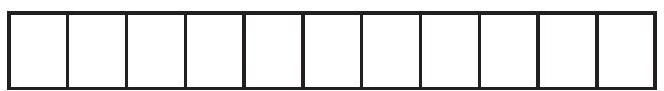
\includegraphics[max width=\textwidth, center]{2024_11_21_e4133e8110fdcfbbacbfg-01(1)}

\section*{ZADANIA ZAMKNIĘTE}
W zadaniach 1.-25. wybierz i zaznacz jedną poprawną odpowiedź.

\section*{Zadanie 1. (0-1)}
Liczba \(a=8^{23} \cdot 4^{17}\) jest równa liczbie:\\
A. \(2^{103}\)\\
B. \(4^{63}\)\\
C. \(2^{59}\)\\
D. \(32^{40}\)

\section*{Zadanie 2. (0-1)}
Liczbą wymierną jest liczba:\\
A. \(36^{\frac{2}{3}}\)\\
B. \(36^{\frac{3}{2}}\)\\
C. \(36^{\frac{1}{4}}\)\\
D. \(36^{\frac{3}{4}}\)

Zadanie 3. (0-1)\\
Wyrażenie \((\sqrt{7}-\sqrt{3})^{2}\) jest równe:\\
A. 44\\
B. 10\\
C. \(10-2 \sqrt{21}\)\\
D. \(10-2 \sqrt{10}\)

\section*{Zadanie 4. (0-1)}
Funkcja \(f(x)=(x+6)^{2}\) ma:\\
A. jedno miejsce zerowe: 6\\
B. jedno miejsce zerowe: -6\\
C. dwa miejsca zerowe: \(6,-6\)\\
D. zero miejsc zerowych

\section*{Zadanie 5. (0-1)}
Tangens kąta ostrego w trójkącie prostokątnym jest równy \(\frac{3}{4}\), a przeciwprostokątna ma długość 30. Krótsza przyprostokątna trójkąta ma długość:\\
A. 15\\
B. 18\\
C. 24\\
D. 26

\section*{Zadanie 6. (0-1)}
Jeśli cena towaru najpierw zmniejszyła się o \(10 \%\), a następnie zwiększyła się o \(20 \%\), to po tych dwóch operacjach wyjściowa cena towaru:\\
A. zwiększyła się o \(10 \%\)\\
B. zmniejszyła się o \(10 \%\)\\
C. zwiększyła się o 8\%\\
D. zmniejszyła się o \(8 \%\)

\section*{Zadanie 7. (0-1)}
Maksymalny przedział otwarty, w którym funkcja \(f(x)=-4 x^{2}+16 x-23\) jest rosnąca, to:\\
A. \((-\infty, 2)\)\\
B. \((-\infty,-2)\)\\
C. \((-\infty,-7)\)\\
D. \((7,+\infty)\)

\section*{Zadanie 8. (0-1)}
Zbiór rozwiązań nierówności \(x-\sqrt{3} x>2\) to:\\
A. \((-\infty,-1-\sqrt{3})\)\\
B. \((-\infty,-1+\sqrt{3})\)\\
C. \((-1-\sqrt{3},+\infty)\)\\
D. \((-1+\sqrt{3},+\infty)\)

\section*{BRUDNOPIS (nie podlega ocenie)}
\begin{center}

\includegraphics[max width=\textwidth]{2024_11_21_e4133e8110fdcfbbacbfg-03}
\end{center}

\section*{Zadanie 9. (0-1)}
W okrąg o środku \(O\) wpisano trójkąt ostrokątny \(A B C\). Jeśli \(|A B O|=48^{\circ}\), to:\\
A. \(|\angle A C B|=42^{\circ}\)\\
B. \(|\angle A C B|=48^{\circ}\)\\
C. \(|\angle A C B|=52^{\circ}\)\\
D. \(|\angle A C B|=58^{\circ}\)

Zadanie 10. (0-1)\\
Dany jest ciąg o wyrazie ogólnym \(a_{n}=-3 n+118\). Liczba dodatnich wyrazów tego ciągu jest równa:\\
A. 37\\
B. 38\\
C. 39\\
D. 0

\section*{Zadanie 11. (0-1)}
Liczba miejsc zerowych funkcji \(f(x)=(x-4)^{2}+9\) to:\\
A. 0\\
B. 1\\
C. 2\\
D. 3

\section*{Zadanie 12. (0-1)}
Zbiorem wartości funkcji \(f(x)=2^{x}+3\) jest zbiór:\\
A. wszystkich liczb rzeczywistych\\
B. \((0,+\infty)\)\\
C. \((-3,+\infty)\)\\
D. \((3,+\infty)\)

\section*{Zadanie 13. (0-1)}
W ciągu arytmetycznym pierwszy i drugi wyraz są odpowiednio równe: \(1,-2\). Dziewiąty wyraz tego ciągu jest równy:\\
A. -23\\
B. 23\\
C. -25\\
D. 25

\section*{Zadanie 14. (0-1)}
Prosta o równaniu \(y=4 x+1\) przecina osie układu współrzędnych w punktach:\\
A. \((1,0) \mathrm{i}\left(0, \frac{1}{4}\right)\)\\
B. \((1,0) \mathrm{i}\left(0,-\frac{1}{4}\right)\)\\
C. \((0,1) \mathrm{i}\left(-\frac{1}{4}, 0\right)\)\\
D. \((0,1) \mathrm{i}\left(\frac{1}{4}, 0\right)\)

\section*{Zadanie 15. (0-1)}
Dana jest funkcja \(f(x)=x^{2}+4 x+10\). Prosta \(y=m\) nie ma z wykresem funkcji \(f\) punktów wspólnych. Maksymalny zbiór, do którego należy liczba \(m\), to:\\
A. \((-\infty,-6)\)\\
B. \((-\infty, 6)\)\\
C. \((-2,+\infty)\)\\
D. \((2,+\infty)\)

\section*{Zadanie 16. (0-1)}
Wiadomo, że \(\operatorname{tg} \alpha=5\) i \(\alpha\) jest kątem ostrym. Wówczas wyrażenie \(W=\frac{\sin \alpha-\cos \alpha}{\sin \alpha+\cos \alpha}\) ma wartość:\\
A. \(\frac{1}{3}\)\\
B. \(\frac{2}{3}\)\\
C. \(\frac{3}{2}\)\\
D. \(\frac{3}{1}\)

\section*{Zadanie 17. (0-1)}
Jeżeli stosunek przyprostokątnych w trójkącie prostokątnym jest równy \(\sqrt{3}\), to jeden z kątów ostrych ma miare:\\
A. \(15^{\circ}\)\\
B. \(30^{\circ}\)\\
C. \(45^{\circ}\)\\
D. \(75^{\circ}\)

\section*{BRUDNOPIS (nie podlega ocenie)}
\begin{center}

\includegraphics[max width=\textwidth]{2024_11_21_e4133e8110fdcfbbacbfg-05}
\end{center}

\section*{Zadanie 18. (0-1)}
Kąt wpisany oparty na \(\frac{1}{9}\) okręgu ma miarę:\\
A. \(80^{\circ}\)\\
B. \(40^{\circ}\)\\
C. \(20^{\circ}\)\\
D. \(10^{\circ}\)

\section*{Zadanie 19. (0-1)}
Jeśli \(S=\left(-\frac{1}{2}, \frac{3}{2}\right)\) jest środkiem odcinka \(A B\) i \(A=\left(-\frac{1}{3}, \frac{2}{3}\right)\), to:\\
A. \(B=\left(-\frac{2}{3}, \frac{7}{3}\right)\)\\
B. \(B=\left(\frac{2}{3}, \frac{7}{3}\right)\)\\
C. \(B=\left(-\frac{2}{3},-\frac{7}{3}\right)\)\\
D. \(B=\left(\frac{2}{3},-\frac{7}{3}\right)\)

\section*{Zadanie 20. (0-1)}
Odchylenie standardowe danych: 1, 4, 1, 5, 9, 2, 1, 1 jest równe (z dokładnością do części setnych):\\
A. 7,25\\
B. 2,69\\
C. 5, 75\\
D. 2,40

\section*{Zadanie 21. (0-1)}
Przekątna przekroju osiowego walca jest nachylona do jego płaszczyzny podstawy pod kątem \(45^{\circ}\). Wysokość walca ma długość 8 . Objętość walca jest równa:\\
A. \(216 \pi\)\\
B. \(128 \pi\)\\
C. \(64 \pi\)\\
D. \(32 \pi\)

\section*{Zadanie 22. (0-1)}
Pole trójkąta jest równe 15. Dwa boki mają długości 10 i 6. Kąt między tymi bokami może mieć miarę:\\
A. \(75^{\circ}\)\\
B. \(60^{\circ}\)\\
C. \(45^{\circ}\)\\
D. \(30^{\circ}\)

\section*{Zadanie 23. (0-1)}
Prosta \(l\) ma równanie \(3 x-2 y=7\). Prosta \(k\) prostopadła do prostej \(l\) może mieć równanie:\\
A. \(y=\frac{2}{3} x+1\)\\
B. \(y=-\frac{2}{3} x+1\)\\
C. \(y=\frac{3}{2} x+1\)\\
D. \(y=-\frac{3}{2} x+1\)

Zadanie 24. (0-1)\\
Liczb czterocyfrowych o różnych cyfrach i o parzystej cyfrze tysięcy, setek i dziesiątek jest:\\
A. 4•4•3.7\\
B. \(4 \cdot 4 \cdot 3 \cdot 8\)\\
C. 5•5•4•8\\
D. 4•5•4•9

\section*{Zadanie 25. (0-1)}
Sześcian przecięto płaszczyzną przechodzącą przez dwie równoległe przekątne dolnej i górnej podstawy. Pole otrzymanego przekroju jest równe 16. Pole powierzchni całkowitej sześcianu jest równe:\\
A. \(8 \sqrt{2}\)\\
B. \(32 \sqrt{2}\)\\
C. \(48 \sqrt{2}\)\\
D. \(56 \sqrt{2}\)

\section*{BRUDNOPIS (nie podlega ocenie)}
\begin{center}

\includegraphics[max width=\textwidth]{2024_11_21_e4133e8110fdcfbbacbfg-07}
\end{center}

\section*{ZADANIA OTWARTE}
Rozwiązania zadań 26.-33. należy zapisać w wyznaczonych miejscach pod treścią zadania.

\section*{Zadanie 26. (0-2)}
Sprawdź, czy liczba \(\frac{33}{27}\) jest wyrazem ciągu o wyrazie ogólnym \(a_{n}=\frac{3 n-1}{2 n+5}\).\\

\includegraphics[max width=\textwidth, center]{2024_11_21_e4133e8110fdcfbbacbfg-08}

Zadanie 27. (0-2)\\
Rozwiąż nierówność \(-x^{2}+8 x-20<0\).\\

\includegraphics[max width=\textwidth, center]{2024_11_21_e4133e8110fdcfbbacbfg-09}

Zadanie 28. (0-2)\\
Punkty \(A=(-2,4), B=(6,2)\) są wierzchołkami trójkąta równobocznego. Wyznacz długość wysokości tego trójkąta.

\begin{center}
\begin{tabular}{|c|c|c|c|c|c|c|c|c|c|c|c|c|c|c|c|c|c|c|c|c|c|}
\hline
 &  &  &  &  &  &  &  &  &  &  &  &  &  &  &  &  &  &  &  &  &  \\
\hline
 &  &  &  &  &  &  &  &  &  &  &  &  &  &  &  &  &  &  &  &  &  \\
\hline
 &  &  &  &  &  &  &  &  &  &  &  &  &  &  &  &  &  &  &  &  &  \\
\hline
 &  &  &  &  &  &  &  &  &  &  &  &  &  &  &  &  &  &  &  &  &  \\
\hline
 &  &  &  &  &  &  &  &  &  &  &  &  &  &  &  &  &  &  &  &  &  \\
\hline
 &  &  &  &  &  &  &  &  &  &  &  &  &  &  &  &  &  &  &  &  &  \\
\hline
 &  &  &  &  &  &  &  &  &  &  &  &  &  &  &  &  &  &  &  &  &  \\
\hline
 &  &  &  &  &  &  &  &  &  &  &  &  &  &  &  &  &  &  &  &  &  \\
\hline
 &  &  &  &  &  &  &  &  &  &  &  &  &  &  &  &  &  &  &  &  &  \\
\hline
 &  &  &  &  &  &  &  &  &  &  &  &  &  &  &  &  &  &  &  &  &  \\
\hline
 &  &  &  &  &  &  &  &  &  &  &  &  &  &  &  &  &  &  &  &  &  \\
\hline
 &  &  &  &  &  &  &  &  &  &  &  &  &  &  &  &  &  &  &  &  &  \\
\hline
 &  &  &  &  &  &  &  &  &  &  &  &  &  &  &  &  &  &  &  &  &  \\
\hline
 &  &  &  &  &  &  &  &  &  &  &  &  &  &  &  &  &  &  &  &  &  \\
\hline
 &  &  &  &  &  &  &  &  &  &  &  &  &  &  &  &  &  &  &  &  &  \\
\hline
 &  &  &  &  &  &  &  &  &  &  &  &  &  &  &  &  &  &  &  &  &  \\
\hline
 &  &  &  &  &  &  &  &  &  &  &  &  &  &  &  &  &  &  &  &  &  \\
\hline
 &  &  &  &  &  &  &  &  &  &  &  &  &  &  &  &  &  &  &  &  &  \\
\hline
 &  &  &  &  &  &  &  &  &  &  &  &  &  &  &  &  &  &  &  &  &  \\
\hline
 &  &  &  &  &  &  &  &  &  &  &  &  &  &  &  &  &  &  &  &  &  \\
\hline
 &  &  &  &  &  &  &  &  &  &  &  &  &  &  &  &  &  &  &  &  &  \\
\hline
 &  &  &  &  &  &  &  &  &  &  &  &  &  &  &  &  &  &  &  &  &  \\
\hline
 &  &  &  &  &  &  &  &  &  &  &  &  &  &  &  &  &  &  &  &  &  \\
\hline
 &  &  &  &  &  &  &  &  &  &  &  &  &  &  &  &  &  &  &  &  &  \\
\hline
 &  &  &  &  &  &  &  &  &  &  &  &  &  &  &  &  &  &  &  &  &  \\
\hline
 &  &  &  &  &  &  &  &  &  &  &  &  &  &  &  &  &  &  &  &  &  \\
\hline
 &  &  &  &  &  &  &  &  &  &  &  &  &  &  &  &  &  &  &  &  &  \\
\hline
 &  &  &  &  &  &  &  &  &  &  &  &  &  &  &  &  &  &  &  &  &  \\
\hline
 &  &  &  &  &  &  &  &  &  &  &  &  &  &  &  &  &  &  &  &  &  \\
\hline
 &  &  &  &  &  &  &  &  &  &  &  &  &  &  &  &  &  &  &  &  &  \\
\hline
 &  &  &  &  &  &  &  &  &  &  &  &  &  &  &  &  &  &  &  &  &  \\
\hline
 &  &  &  &  &  &  &  &  &  &  &  &  &  &  &  &  &  &  &  &  &  \\
\hline
 &  &  &  &  &  &  &  &  &  &  &  &  &  &  &  &  &  &  &  &  &  \\
\hline
 &  &  &  &  &  &  &  &  &  &  &  &  &  &  &  &  &  &  &  &  &  \\
\hline
 &  &  &  &  &  &  &  &  &  &  &  &  &  &  &  &  &  &  &  &  &  \\
\hline
 &  &  &  &  &  &  &  &  &  &  &  &  &  &  &  &  &  &  &  &  &  \\
\hline
 &  &  &  &  &  &  &  &  &  &  &  &  &  &  &  &  &  &  &  &  &  \\
\hline
 &  &  &  &  &  &  &  &  &  &  &  &  &  &  &  &  &  &  &  &  &  \\
\hline
 &  &  &  &  &  &  &  &  &  &  &  &  &  &  &  &  &  &  &  &  &  \\
\hline
 &  &  &  &  &  &  &  &  &  &  &  &  &  &  &  &  &  &  &  &  &  \\
\hline
 &  &  &  &  &  &  &  &  &  &  &  &  &  &  &  &  &  &  &  &  &  \\
\hline
 &  &  &  &  &  &  &  &  &  &  &  &  &  &  &  &  &  &  &  &  &  \\
\hline
\end{tabular}
\end{center}

Zadanie 29. (0-2)\\
Wykaż, że dla dowolnych liczb rzeczywistych \(x, y\) prawdziwa jest nierówność \(x^{2}-6 x+y^{2}-4 y+13 \geq 0\).

\begin{center}
\begin{tabular}{|c|c|c|c|c|c|c|c|c|c|c|c|c|c|c|c|c|c|c|c|c|}
\hline
 &  &  &  &  &  &  &  &  &  &  &  &  &  &  &  &  &  &  &  &  \\
\hline
 &  &  &  &  &  &  &  &  &  &  &  &  &  &  &  &  &  &  &  &  \\
\hline
 &  &  &  &  &  &  &  &  &  &  &  &  &  &  &  &  &  &  &  &  \\
\hline
 &  &  &  &  &  &  &  &  &  &  &  &  &  &  &  &  &  &  &  &  \\
\hline
 &  &  &  &  &  &  &  &  &  &  &  &  &  &  &  &  &  &  &  &  \\
\hline
 &  &  &  &  &  &  &  &  &  &  &  &  &  &  &  &  &  &  &  &  \\
\hline
 &  &  &  &  &  &  &  &  &  &  &  &  &  &  &  &  &  &  &  &  \\
\hline
 &  &  &  &  &  &  &  &  &  &  &  &  &  &  &  &  &  &  &  &  \\
\hline
 &  &  &  &  &  &  &  &  &  &  &  &  &  &  &  &  &  &  &  &  \\
\hline
 &  &  &  &  &  &  &  &  &  &  &  &  &  &  &  &  &  &  &  &  \\
\hline
 &  &  &  &  &  &  &  &  &  &  &  &  &  &  &  &  &  &  &  &  \\
\hline
 &  &  &  &  &  &  &  &  &  &  &  &  &  &  &  &  &  &  &  &  \\
\hline
 &  &  &  &  &  &  &  &  &  &  &  &  &  &  &  &  &  &  &  &  \\
\hline
 &  &  &  &  &  &  &  &  &  &  &  &  &  &  &  &  &  &  &  &  \\
\hline
 &  &  &  &  &  &  &  &  &  &  &  &  &  &  &  &  &  &  &  &  \\
\hline
 &  &  &  &  &  &  &  &  &  &  &  &  &  &  &  &  &  &  &  &  \\
\hline
 &  &  &  &  &  &  &  &  &  &  &  &  &  &  &  &  &  &  &  &  \\
\hline
 &  &  &  &  &  &  &  &  &  &  &  &  &  &  &  &  &  &  &  &  \\
\hline
 &  &  &  &  &  &  &  &  &  &  &  &  &  &  &  &  &  &  &  &  \\
\hline
 &  &  &  &  &  &  &  &  &  &  &  &  &  &  &  &  &  &  &  &  \\
\hline
 &  &  &  &  &  &  &  &  &  &  &  &  &  &  &  &  &  &  &  &  \\
\hline
 &  &  &  &  &  &  &  &  &  &  &  &  &  &  &  &  &  &  &  &  \\
\hline
 &  &  &  &  &  &  &  &  &  &  &  &  &  &  &  &  &  &  &  &  \\
\hline
 &  &  &  &  &  &  &  &  &  &  &  &  &  &  &  &  &  &  &  &  \\
\hline
 &  &  &  &  &  &  &  &  &  &  &  &  &  &  &  &  &  &  &  &  \\
\hline
 &  &  &  &  &  &  &  &  &  &  &  &  &  &  &  &  &  &  &  &  \\
\hline
 &  &  &  &  &  &  &  &  &  &  &  &  &  &  &  &  &  &  &  &  \\
\hline
 &  &  &  &  &  &  &  &  &  &  &  &  &  &  &  &  &  &  &  &  \\
\hline
 &  &  &  &  &  &  &  &  &  &  &  &  &  &  &  &  &  &  &  &  \\
\hline
 &  &  &  &  &  &  &  &  &  &  &  &  &  &  &  &  &  &  &  &  \\
\hline
 &  &  &  &  &  &  &  &  &  &  &  &  &  &  &  &  &  &  &  &  \\
\hline
 &  &  &  &  &  &  &  &  &  &  &  &  &  &  &  &  &  &  &  &  \\
\hline
 &  &  &  &  &  &  &  &  &  &  &  &  &  &  &  &  &  &  &  &  \\
\hline
 &  &  &  &  &  &  &  &  &  &  &  &  &  &  &  &  &  &  &  &  \\
\hline
 &  &  &  &  &  &  &  &  &  &  &  &  &  &  &  &  &  &  &  &  \\
\hline
 &  &  &  &  &  &  &  &  &  &  &  &  &  &  &  &  &  &  &  &  \\
\hline
 &  &  &  &  &  &  &  &  &  &  &  &  &  &  &  &  &  &  &  &  \\
\hline
 &  &  &  &  &  &  &  &  &  &  &  &  &  &  &  &  &  &  &  &  \\
\hline
 &  &  &  &  &  &  &  &  &  &  &  &  &  &  &  &  &  &  &  &  \\
\hline
 &  &  &  &  &  &  &  &  &  &  &  &  &  &  &  &  &  &  &  &  \\
\hline
 &  &  &  &  &  &  &  &  &  &  &  &  &  &  &  &  &  &  &  &  \\
\hline
 &  &  &  &  &  &  &  &  &  &  &  &  &  &  &  &  &  &  &  &  \\
\hline
\end{tabular}
\end{center}

Zadanie 30. (0-2)\\
Dany jest kwadrat o boku \(a=6\). W ten kwadrat wpisano trójkąt równoboczny w ten sposób, że jeden wierzchołek trójkąta jest wierzchołkiem kwadratu, a przeciwległy bok trójkąta jest równoległy do przekątnej kwadratu (patrz rysunek). Wykaż, że bok trójkąta jest równy \(6(\sqrt{6}-\sqrt{2})\).\\

\includegraphics[max width=\textwidth, center]{2024_11_21_e4133e8110fdcfbbacbfg-12}

\begin{center}
\begin{tabular}{|c|c|c|c|c|c|c|c|c|c|c|c|c|c|c|c|c|c|c|c|c|c|c|c|c|c|c|c|c|c|}
\hline
 &  &  &  &  &  &  &  &  &  &  &  &  &  &  &  &  &  &  &  &  &  &  &  &  &  &  &  &  &  \\
\hline
 &  &  &  &  &  &  &  &  &  &  &  &  &  &  &  &  &  &  &  &  &  &  &  &  &  &  &  &  &  \\
\hline
 &  &  &  &  &  &  &  &  &  &  &  &  &  &  &  &  &  &  &  &  &  &  &  &  &  &  &  &  &  \\
\hline
 &  &  &  &  &  &  &  &  &  &  &  &  &  &  &  &  &  &  &  &  &  &  &  &  &  &  &  &  &  \\
\hline
 &  &  &  &  &  &  &  &  &  &  &  &  &  &  &  &  &  &  &  &  &  &  &  &  &  &  &  &  &  \\
\hline
 &  &  &  &  &  &  &  &  &  &  &  &  &  &  &  &  &  &  &  &  &  &  &  &  &  &  &  &  &  \\
\hline
 &  &  &  &  &  &  &  &  &  &  &  &  &  &  &  &  &  &  &  &  &  &  &  &  &  &  &  &  &  \\
\hline
到 &  &  &  &  &  &  &  &  &  &  &  &  &  &  &  &  &  &  &  &  &  &  &  &  &  &  &  &  &  \\
\hline
 &  &  &  &  &  &  &  &  &  &  &  &  &  &  &  &  &  &  &  &  &  &  &  &  &  &  &  &  &  \\
\hline
- &  &  &  &  &  &  &  &  &  &  &  &  &  &  &  &  &  &  &  &  &  &  &  &  &  &  &  &  &  \\
\hline
 &  &  &  &  &  &  &  &  &  &  &  &  &  &  &  &  &  &  &  &  &  &  &  &  &  &  &  &  &  \\
\hline
 &  &  &  &  &  &  &  &  &  &  &  &  &  &  &  &  &  &  &  &  &  &  &  &  &  &  &  &  &  \\
\hline
 &  &  &  &  &  &  &  &  &  &  &  &  &  &  &  &  &  &  &  &  &  &  &  &  &  &  &  &  &  \\
\hline
 &  &  &  &  &  &  &  &  &  &  &  &  &  &  &  &  &  &  &  &  &  &  &  &  &  &  &  &  &  \\
\hline
 &  &  &  &  &  &  &  &  &  &  &  &  &  &  &  &  &  &  &  &  &  &  &  &  &  &  &  &  &  \\
\hline
- &  &  &  &  &  &  &  &  &  &  &  &  &  &  &  &  &  &  &  &  &  &  &  &  &  &  &  &  &  \\
\hline
 &  &  &  &  &  &  &  &  &  &  &  &  &  &  &  &  &  &  &  &  &  &  &  &  &  &  &  &  &  \\
\hline
 &  &  &  &  &  &  &  &  &  &  &  &  &  &  &  &  &  &  &  &  &  &  &  &  &  &  &  &  &  \\
\hline
 &  &  &  &  &  &  &  &  &  &  &  &  &  &  &  &  &  &  &  &  &  &  &  &  &  &  &  &  &  \\
\hline
- &  &  &  &  &  &  &  &  &  &  &  &  &  &  &  &  &  &  &  &  &  &  &  &  &  &  &  &  &  \\
\hline
 &  &  &  &  &  &  &  &  &  &  &  &  &  &  &  &  &  &  &  &  &  &  &  &  &  &  &  &  &  \\
\hline
 &  &  &  &  &  &  &  &  &  &  &  &  &  &  &  &  &  &  &  &  &  &  &  &  &  &  &  &  &  \\
\hline
 &  &  &  &  &  &  &  &  &  &  &  &  &  &  &  &  &  &  &  &  &  &  &  &  &  &  &  &  &  \\
\hline
 &  &  &  &  &  &  &  &  &  &  &  &  &  &  &  &  &  &  &  &  &  &  &  &  &  &  &  &  &  \\
\hline
 &  &  &  &  &  &  &  &  &  &  &  &  &  &  &  &  &  &  &  &  &  &  &  &  &  &  &  &  &  \\
\hline
 &  &  &  &  &  &  &  &  &  &  &  &  &  &  &  &  &  &  &  &  &  &  &  &  &  &  &  &  &  \\
\hline
- &  &  &  &  &  &  &  &  &  &  &  &  &  &  &  &  &  &  &  &  &  &  &  &  &  &  &  &  &  \\
\hline
 &  &  &  &  &  &  &  &  &  &  &  &  &  &  &  &  &  &  &  &  &  &  &  &  &  &  &  &  &  \\
\hline
\end{tabular}
\end{center}

\section*{Zadanie 31. (0-4)}
Dana jest funkcja określona wzorem \(f(x)=a x^{2}+b x+c\). Wartość największa funkcji jest równa 10. Funkcja jest rosnąca jedynie w przedziale \((-\infty, 2)\), a do jej wykresu należy punkt \(A=(4,-2)\). Wyznacz wartości współczynników \(a, b, c\).

\begin{center}
\begin{tabular}{|c|c|c|c|c|c|c|c|c|c|c|c|c|c|c|c|c|c|c|c|c|c|}
\hline
 &  &  &  &  &  &  &  &  &  &  &  &  &  &  &  &  &  &  &  &  &  \\
\hline
 &  &  &  &  &  &  &  &  &  &  &  &  &  &  &  &  &  &  &  &  &  \\
\hline
 &  &  &  &  &  &  &  &  &  &  &  &  &  &  &  &  &  &  &  &  &  \\
\hline
 &  &  &  &  &  &  &  &  &  &  &  &  &  &  &  &  &  &  &  &  &  \\
\hline
 &  &  &  &  &  &  &  &  &  &  &  &  &  &  &  &  &  &  &  &  &  \\
\hline
 &  &  &  &  &  &  &  &  &  &  &  &  &  &  &  &  &  &  &  &  &  \\
\hline
 &  &  &  &  &  &  &  &  &  &  &  &  &  &  &  &  &  &  &  &  &  \\
\hline
 &  &  &  &  &  &  &  &  &  &  &  &  &  &  &  &  &  &  &  &  &  \\
\hline
 &  &  &  &  &  &  &  &  &  &  &  &  &  &  &  &  &  &  &  &  &  \\
\hline
 &  &  &  &  &  &  &  &  &  &  &  &  &  &  &  &  &  &  &  &  &  \\
\hline
 &  &  &  &  &  &  &  &  &  &  &  &  &  &  &  &  &  &  &  &  &  \\
\hline
 &  &  &  &  &  &  &  &  &  &  &  &  &  &  &  &  &  &  &  &  &  \\
\hline
 &  &  &  &  &  &  &  &  &  &  &  &  &  &  &  &  &  &  &  &  &  \\
\hline
 &  &  &  &  &  &  &  &  &  &  &  &  &  &  &  &  &  &  &  &  &  \\
\hline
 &  &  &  &  &  &  &  &  &  &  &  &  &  &  &  &  &  &  &  &  &  \\
\hline
 &  &  &  &  &  &  &  &  &  &  &  &  &  &  &  &  &  &  &  &  &  \\
\hline
 &  &  &  &  &  &  &  &  &  &  &  &  &  &  &  &  &  &  &  &  &  \\
\hline
 &  &  &  &  &  &  &  &  &  &  &  &  &  &  &  &  &  &  &  &  &  \\
\hline
 &  &  &  &  &  &  &  &  &  &  &  &  &  &  &  &  &  &  &  &  &  \\
\hline
 &  &  &  &  &  &  &  &  &  &  &  &  &  &  &  &  &  &  &  &  &  \\
\hline
 &  &  &  &  &  &  &  &  &  &  &  &  &  &  &  &  &  &  &  &  &  \\
\hline
 &  &  &  &  &  &  &  &  &  &  &  &  &  &  &  &  &  &  &  &  &  \\
\hline
 &  &  &  &  &  &  &  &  &  &  &  &  &  &  &  &  &  &  &  &  &  \\
\hline
 &  &  &  &  &  &  &  &  &  &  &  &  &  &  &  &  &  &  &  &  &  \\
\hline
 &  &  &  &  &  &  &  &  &  &  &  &  &  &  &  &  &  &  &  &  &  \\
\hline
 &  &  &  &  &  &  &  &  &  &  &  &  &  &  &  &  &  &  &  &  &  \\
\hline
 &  &  &  &  &  &  &  &  &  &  &  &  &  &  &  &  &  &  &  &  &  \\
\hline
 &  &  &  &  &  &  &  &  &  &  &  &  &  &  &  &  &  &  &  &  &  \\
\hline
 &  &  &  &  &  &  &  &  &  &  &  &  &  &  &  &  &  &  &  &  &  \\
\hline
 &  &  &  &  &  &  &  &  &  &  &  &  &  &  &  &  &  &  &  &  &  \\
\hline
 &  &  &  &  &  &  &  &  &  &  &  &  &  &  &  &  &  &  &  &  &  \\
\hline
 &  &  &  &  &  &  &  &  &  &  &  &  &  &  &  &  &  &  &  &  &  \\
\hline
 &  &  &  &  &  &  &  &  &  &  &  &  &  &  &  &  &  &  &  &  &  \\
\hline
 &  &  &  &  &  &  &  &  &  &  &  &  &  &  &  &  &  &  &  &  &  \\
\hline
 &  &  &  &  &  &  &  &  &  &  &  &  &  &  &  &  &  &  &  &  &  \\
\hline
 &  &  &  &  &  &  &  &  &  &  &  &  &  &  &  &  &  &  &  &  &  \\
\hline
 &  &  &  &  &  &  &  &  &  &  &  &  &  &  &  &  &  &  &  &  &  \\
\hline
 &  &  &  &  &  &  &  &  &  &  &  &  &  &  &  &  &  &  &  &  &  \\
\hline
 &  &  &  &  &  &  &  &  &  &  &  &  &  &  &  &  &  &  &  &  &  \\
\hline
 &  &  &  &  &  &  &  &  &  &  &  &  &  &  &  &  &  &  &  &  &  \\
\hline
 &  &  &  &  &  &  &  &  &  &  &  &  &  &  &  &  &  &  &  &  &  \\
\hline
\end{tabular}
\end{center}

\section*{Zadanie 32. (0-5)}
Pierwszy wyraz ciągu arytmetycznego jest równy 4, a suma kwadratów wyrazu drugiego, czwartego i siódmego jest równa 702. Wyznacz ogólny wyraz tego ciągu.\\

\includegraphics[max width=\textwidth, center]{2024_11_21_e4133e8110fdcfbbacbfg-14}

\section*{Zadanie 33. (0-6)}
Dany jest ostrosłup prawidłowy trójkątny. Promień okręgu wpisanego w podstawę jest równy 6. Ściana boczna tworzy z płaszczyzną podstawy kąt \(60^{\circ}\). Oblicz objętość i pole powierzchni bocznej bryły.

\begin{center}
\begin{tabular}{|c|c|c|c|c|c|c|c|c|c|c|c|c|c|c|c|c|c|c|c|c|c|c|}
\hline
 &  &  &  &  &  &  &  &  &  &  &  &  &  &  &  &  &  &  &  &  &  &  \\
\hline
 &  &  &  &  &  &  &  &  &  &  &  &  &  &  &  &  &  &  &  &  &  &  \\
\hline
 &  &  &  &  &  &  &  &  &  &  &  &  &  &  &  &  &  &  &  &  &  &  \\
\hline
 &  &  &  &  &  &  &  &  &  &  &  &  &  &  &  &  &  &  &  &  &  &  \\
\hline
 &  &  &  &  &  &  &  &  &  &  &  &  &  &  &  &  &  &  &  &  &  &  \\
\hline
 &  &  &  &  &  &  &  &  &  &  &  &  &  &  &  &  &  &  &  &  &  &  \\
\hline
 &  &  &  &  &  &  &  &  &  &  &  &  &  &  &  &  &  &  &  &  &  &  \\
\hline
 &  &  &  &  &  &  &  &  &  &  &  &  &  &  &  &  &  &  &  &  &  &  \\
\hline
 &  &  &  &  &  &  &  &  &  &  &  &  &  &  &  &  &  &  &  &  &  &  \\
\hline
 &  &  &  &  &  &  &  &  &  &  &  &  &  &  &  &  &  &  &  &  &  &  \\
\hline
 &  &  &  &  &  &  &  &  &  &  &  &  &  &  &  &  &  &  &  &  &  &  \\
\hline
 &  &  &  &  &  &  &  &  &  &  &  &  &  &  &  &  &  &  &  &  &  &  \\
\hline
 &  &  &  &  &  &  &  &  &  &  &  &  &  &  &  &  &  &  &  &  &  &  \\
\hline
 &  &  &  &  &  &  &  &  &  &  &  &  &  &  &  &  &  &  &  &  &  &  \\
\hline
 &  &  &  &  &  &  &  &  &  &  &  &  &  &  &  &  &  &  &  &  &  &  \\
\hline
 &  &  &  &  &  &  &  &  &  &  &  &  &  &  &  &  &  &  &  &  &  &  \\
\hline
 &  &  &  &  &  &  &  &  &  &  &  &  &  &  &  &  &  &  &  &  &  &  \\
\hline
 & 
\includegraphics[max width=\textwidth]{2024_11_21_e4133e8110fdcfbbacbfg-15(4)}
 &  &  &  &  &  &  &  &  &  &  &  &  &  &  &  &  &  &  &  &  &  \\
\hline
 &  &  &  &  &  &  &  &  &  &  &  &  &  &  &  &  &  &  &  &  &  &  \\
\hline
 &  &  &  &  &  &  &  &  &  &  &  &  &  &  &  &  &  &  &  &  &  &  \\
\hline
 &  &  &  &  &  &  &  &  &  &  &  &  &  &  &  &  &  &  &  &  &  &  \\
\hline
 & 
\includegraphics[max width=\textwidth]{2024_11_21_e4133e8110fdcfbbacbfg-15(6)}
 &  &  &  &  &  &  &  &  &  &  &  &  &  &  &  &  &  &  &  &  &  \\
\hline
 & 
\includegraphics[max width=\textwidth]{2024_11_21_e4133e8110fdcfbbacbfg-15}
 &  &  &  &  &  &  &  &  &  &  &  &  &  &  &  &  &  &  &  &  &  \\
\hline
 & 
\includegraphics[max width=\textwidth]{2024_11_21_e4133e8110fdcfbbacbfg-15(1)}
 &  &  &  &  &  &  &  &  &  &  &  &  &  &  &  &  &  &  &  &  &  \\
\hline
 & 
\includegraphics[max width=\textwidth]{2024_11_21_e4133e8110fdcfbbacbfg-15(5)}
 &  &  &  &  &  &  &  &  &  &  &  &  &  &  &  &  &  &  &  &  &  \\
\hline
 & 
\includegraphics[max width=\textwidth]{2024_11_21_e4133e8110fdcfbbacbfg-15(3)}
 &  &  &  &  &  &  &  &  &  &  &  &  &  &  &  &  &  &  &  &  &  \\
\hline
 & ■ &  &  &  &  &  &  &  &  &  &  &  &  &  &  &  &  &  &  &  &  &  \\
\hline
 & - &  &  &  &  &  &  &  &  &  &  &  &  &  &  &  &  &  &  &  &  &  \\
\hline
 &  &  &  &  &  &  &  &  &  &  &  &  &  &  &  &  &  &  &  &  &  &  \\
\hline
 & 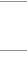
\includegraphics[max width=\textwidth]{2024_11_21_e4133e8110fdcfbbacbfg-15(2)}
 &  &  &  &  &  &  &  &  &  &  &  &  &  &  &  &  &  &  &  &  &  \\
\hline
 &  &  &  &  &  &  &  &  &  &  &  &  &  &  &  &  &  &  &  &  &  &  \\
\hline
 &  &  &  &  &  &  &  &  &  &  &  &  &  &  &  &  &  &  &  &  &  &  \\
\hline
 &  &  &  &  &  &  &  &  &  &  &  &  &  &  &  &  &  &  &  &  &  &  \\
\hline
 & - &  &  &  &  &  &  &  &  &  &  &  &  &  &  &  &  &  &  &  &  &  \\
\hline
 &  &  &  &  &  &  &  &  &  &  &  &  &  &  &  &  &  &  &  &  &  &  \\
\hline
 &  &  &  &  &  &  &  &  &  &  &  &  &  &  &  &  &  &  &  &  &  &  \\
\hline
 &  &  &  &  &  &  &  &  &  &  &  &  &  &  &  &  &  &  &  &  &  &  \\
\hline
 &  &  &  &  &  &  &  &  &  &  &  &  &  &  &  &  &  &  &  &  &  &  \\
\hline
 &  &  &  &  &  &  &  &  &  &  &  &  &  &  &  &  &  &  &  &  &  &  \\
\hline
 &  &  &  &  &  &  &  &  &  &  &  &  &  &  &  &  &  &  &  &  &  &  \\
\hline
 &  &  &  &  &  &  &  &  &  &  &  &  &  &  &  &  &  &  &  &  &  &  \\
\hline
 &  &  &  &  &  &  &  &  &  &  &  &  &  &  &  &  &  &  &  &  &  &  \\
\hline
\end{tabular}
\end{center}

\section*{BRUDNOPIS (nie podlega ocenie)}
\begin{center}

\includegraphics[max width=\textwidth]{2024_11_21_e4133e8110fdcfbbacbfg-16}
\end{center}


\end{document}